\section{Durchführung}
\label{sec:Durchführung}
Zunächst wird eine Schwingkreis wie in Abbildung \ref{fig:aufbau1} aufgebaut.
Als erstes wird die Zeitabhängigkeit der Amplitude bei einer gedämpften Schwingung
gemessen, um daraus den effektiven Dämpfungswiderstand zu berechnen.
\begin{figure}
  \centering
  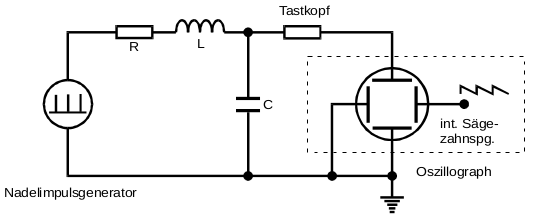
\includegraphics[width=0.9\textwidth]{aufbau1.png}
  \caption{Aufbau eines RLC-Schwingkreises mit einem Nadelimpulsgenerator. Die
  Kondensatorspannung wird mit einem hochohmigen Tastkopf abgegriffen und mit
  einem Speicheroszilloskop dargestellt\cite{sample}.}
  \label{fig:aufbau1}
\end{figure}
Nun wird der Widerstand $R$ durch einen variablen Widerstand ersetzt, welcher zu
Beginn der Messung auf seinen Maximalwert von $10 \si{\kilo\ohm}$ eingestellt wird
und dann so weit verringert wird, bis gerade noch kein Überschwingen eintritt,
also genau der aperiodische Grenzfall erreicht ist. Der eingestellte Wert des
variablen Widerstandes entspricht nun $R_\symup{ap}$.

Als nächstes wird ein Schaltkreis wie in Abbildung \ref{fig:aufbau2} aufgebaut.
Der Nadelimpulsgenerator wird durch einen Sinunsgenerator ersetzt und es wird
sowohl die Erregerspannung $U_\symup{S}$, als auch die Kondensatorspannung
$U_\symup{C}$ mit dem Zweikanaloszilloskoph dargestellt.
\begin{figure}
  \centering
  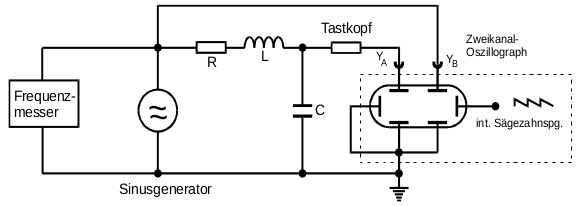
\includegraphics[width=0.9\textwidth]{aufbau2.png}
  \caption{Schaltung mit einem Sinusgenerator und einem RLC-Schwingkreis zur
  Messung der Frequenzabhängigkeit der Kondensatorspannung sowie der
  Phasenverschiebung zwischen Erregerspannung und Kondensatorspannung, welche mit
  einem Zweikanaloszilloskop dargestellt werden\cite{sample}.}
  \label{fig:aufbau2}
\end{figure}
Es werden nun Messwerte für die Kondensatorspannung $U_\symup{C}$ und die
Phasenverschiebung zwischen der Erregerspannung $U_\symup{S}$ und der
Kondensatorspannung $U_\symup{C}$ bei verschiedenen Frequenzen aufgenommen. Um
die Phasendifferenz berechnen zu können werden die Differenzen der Nulldurchgänge
gemessen.
